% Options for packages loaded elsewhere
\PassOptionsToPackage{unicode}{hyperref}
\PassOptionsToPackage{hyphens}{url}
%
\documentclass[
  12pt,a4paper,lualatex,ja=standard]{bxjsarticle}
\usepackage{lmodern}
\usepackage{amsmath}
\usepackage{ifxetex,ifluatex}
\ifnum 0\ifxetex 1\fi\ifluatex 1\fi=0 % if pdftex
  \usepackage[T1]{fontenc}
  \usepackage[utf8]{inputenc}
  \usepackage{textcomp} % provide euro and other symbols
  \usepackage{amssymb}
\else % if luatex or xetex
  \usepackage{unicode-math}
  \defaultfontfeatures{Scale=MatchLowercase}
  \defaultfontfeatures[\rmfamily]{Ligatures=TeX,Scale=1}
\fi
% Use upquote if available, for straight quotes in verbatim environments
\IfFileExists{upquote.sty}{\usepackage{upquote}}{}
\IfFileExists{microtype.sty}{% use microtype if available
  \usepackage[]{microtype}
  \UseMicrotypeSet[protrusion]{basicmath} % disable protrusion for tt fonts
}{}
\makeatletter
\@ifundefined{KOMAClassName}{% if non-KOMA class
  \IfFileExists{parskip.sty}{%
    \usepackage{parskip}
  }{% else
    \setlength{\parindent}{0pt}
    \setlength{\parskip}{6pt plus 2pt minus 1pt}}
}{% if KOMA class
  \KOMAoptions{parskip=half}}
\makeatother
\usepackage{xcolor}
\IfFileExists{xurl.sty}{\usepackage{xurl}}{} % add URL line breaks if available
\IfFileExists{bookmark.sty}{\usepackage{bookmark}}{\usepackage{hyperref}}
\hypersetup{
  hidelinks,
  pdfcreator={LaTeX via pandoc}}
\urlstyle{same} % disable monospaced font for URLs
\usepackage{graphicx}
\makeatletter
\def\maxwidth{\ifdim\Gin@nat@width>\linewidth\linewidth\else\Gin@nat@width\fi}
\def\maxheight{\ifdim\Gin@nat@height>\textheight\textheight\else\Gin@nat@height\fi}
\makeatother
% Scale images if necessary, so that they will not overflow the page
% margins by default, and it is still possible to overwrite the defaults
% using explicit options in \includegraphics[width, height, ...]{}
\setkeys{Gin}{width=\maxwidth,height=\maxheight,keepaspectratio}
% Set default figure placement to htbp
\makeatletter
\def\fps@figure{htbp}
\makeatother
\setlength{\emergencystretch}{3em} % prevent overfull lines
\providecommand{\tightlist}{%
  \setlength{\itemsep}{0pt}\setlength{\parskip}{0pt}}
\setcounter{secnumdepth}{5}
\usepackage{indentfirst}
\parindent = 1em
\usepackage{dcolumn}
\newcolumntype{.}{D{.}{.}{-1}}
\usepackage{caption}
\captionsetup[table]{name=表}
\captionsetup[figure]{name=図}
\usepackage{hyperref}
\pagestyle{empty}
\usepackage{multicol}
\usepackage{ascmac}
\setpagelayout*{top=10truemm,bottom=30truemm,left=10truemm,right=10truemm}
\usepackage{tikz}
\usetikzlibrary{arrows.meta,decorations,decorations.pathreplacing,arrows,calc}
\usepackage{tabstackengine}
\usepackage{xcolor}
\usepackage{rotating}
\usepackage{txfonts}
\usepackage{fancybox}
\usepackage{dashbox}
\usepackage{tcolorbox}
\tcbuselibrary{theorems,skins}
\usepackage{siunitx}
\usepackage{framed}
\usepackage{enumerate}
\usepackage{lastpage}
\usepackage{pgfplots}
\pgfplotsset{compat=1.15}
\usepackage{mathrsfs}
\ifluatex
  \usepackage{selnolig}  % disable illegal ligatures
\fi

\author{}
\date{\vspace{-2.5em}}

\begin{document}

\renewcommand{\thefootnote}{}
\newcounter{kaunta}
\renewcommand{\thekaunta}{\arabic{kaunta}}
\newcommand{\kaunta}{\refstepcounter{kaunta}%
\thekaunta}
\def\question{\noindent\fbox{\large\makebox[1em]{\text{\kaunta}}} \hspace{1pt}}
\newcounter{skaunta}
\renewcommand{\theskaunta}{\arabic{skaunta}}
\newcommand{\skaunta}{\refstepcounter{skaunta}%
\theskaunta}
\def\squestion{(\text{\skaunta})\hspace{2.5pt}}
\newcommand{\maru}[1]{\raise0.2ex\hbox{\textcircled{\scriptsize{#1}}}}
\newcommand{\jsim}{\mathrel{\text{∽}}}
\newcommand{\jpara}{/\!/}
\newcounter{kurankaunta}
\renewcommand{\thekurankaunta}{\arabic{kurankaunta}}
\newcommand{\kurankaunta}{\refstepcounter{kurankaunta}%
\thekurankaunta}

\newcounter{kcounter}
\setcounter{kcounter}{0}
\newcommand{\kana}{\refstepcounter{kcounter}\ifthenelse{\value{kcounter}=1}{ア}{\ifthenelse{\value{kcounter}=2}{イ}{\ifthenelse{\value{kcounter}=3}{ウ}{\ifthenelse{\value{kcounter}=4}{エ}{\ifthenelse{\value{kcounter}=5}{オ} {\ifthenelse{\value{kcounter}=6}{カ}{\ifthenelse{\value{kcounter}=7}{キ}{\ifthenelse{\value{kcounter}=8}{ク}{\ifthenelse{\value{kcounter}=9}{ケ}{\ifthenelse{\value{kcounter}=10}{コ}{\ifthenelse{\value{kcounter}=11}{サ}{\ifthenelse{\value{kcounter}=12}{シ}{\ifthenelse{\value{kcounter}=13}{ス}{\ifthenelse{\value{kcounter}=14}{セ}{\ifthenelse{\value{kcounter}=15}{ソ}{\ifthenelse{\value{kcounter}=16}{タ}{\ifthenelse{\value{kcounter}=17}{チ}{\ifthenelse{\value{kcounter}=18}{ツ}{\ifthenelse{\value{kcounter}=19}{テ}{\ifthenelse{\value{kcounter}=20}{ト}{\ifthenelse{\value{kcounter}=21}{ナ}{\ifthenelse{\value{kcounter}=22}{ニ}{\ifthenelse{\value{kcounter}=23}{ヌ}{\ifthenelse{\value{kcounter}=24}{ネ}{\ifthenelse{\value{kcounter}=25}{ノ}{\ifthenelse{\value{kcounter}=26}{ハ}{\ifthenelse{\value{kcounter}=27}{ヒ}{\ifthenelse{\value{kcounter}=28}{フ}{\ifthenelse{\value{kcounter}=29}{ヘ}{\ifthenelse{\value{kcounter}=30}{ホ}{\ifthenelse{\value{kcounter}=31}{マ}{\ifthenelse{\value{kcounter}=32}{ミ}{\ifthenelse{\value{kcounter}=33}{ム}{\ifthenelse{\value{kcounter}=34}{メ}{\ifthenelse{\value{kcounter}=35}{モ}{\ifthenelse{\value{kcounter}=36}{ヤ}{\ifthenelse{\value{kcounter}=37}{ユ}{\ifthenelse{\value{kcounter}=38}{ヨ}{\ifthenelse{\value{kcounter}=39}{ラ}{\ifthenelse{\value{kcounter}=40}{リ}{\ifthenelse{\value{kcounter}=41}{ル}{\ifthenelse{\value{kcounter}=42}{レ}{\ifthenelse{\value{kcounter}=43}{ロ}{\ifthenelse{\value{kcounter}=44}{ワ}{・}}}}}}}}}}}}}}}}}}}}}}}}}}}}}}}}}}}}}}}}}}}}}

\newcommand{\kuran}[1]{\framebox[1.5cm][c]{\maru{\kana}}}
\newcommand{\sukuran}[1]{\framebox[1.5cm][c]{\maru{\kurankaunta}}}

\newcommand{\degre}{\ensuremath{^\circ}}

\newcommand{\myarc}[1]{
   \tikz [baseline = (N.base), every node/.style={}] {
      \node [inner sep = 0pt] (N) {$\mathrm{#1}$};
      \draw [line width = 0.4pt] plot [smooth, tension=1.3] coordinates {
         ($(N.north west) + (0.1ex,0)$)
         ($(N.north)      + (0,0.5ex)$)
         ($(N.north east) + (0,0)$)
      };
   }
}

\makeatletter
\newenvironment{figurehere}{\def\@captype{figure}}{}
\makeatother

\newcommand{\haiten}[1]{%
\begin{flushright}%
\footnotesize{<#1>}%
\end{flushright}%
}

\newcommand{\goku}[1]{\fbox{\phantom{\text{#1}} \quad}}

\newgeometry{top=10truemm,bottom=10truemm,left=20truemm,right=20truemm}

\thispagestyle{empty}
\begin{center}
\phantom{empty}

\vspace{60truemm}

\hspace{4em} {\HUGE\gtfamily\bfseries 数\hspace{2em}学}\hspace{1em}{\large \gtfamily \bfseries ($\mathbf{1}$年)}\\

\vspace{15truemm}

\hspace{2.5em}{\large \gtfamily \bfseries 春休みの宿題}

\vspace{150truemm}


\end{center}

\begin{center}
{\large \underline{\hspace{30mm}組 \hspace{30mm}番 \hspace{15mm} 名前 \hspace{60mm}}}
\end{center}

\newpage

\pagestyle{plain}
\pagenumbering{arabic}

\begin{flushleft}

\noindent\fbox{\large\makebox[1em]{\text{\refstepcounter{kaunta}%
\arabic{kaunta}}}} \hspace{1pt}次の数のうち、素数であるものを答えなさい。

$-5$, \hspace{5mm} 0, \hspace{5mm} 3, \hspace{5mm} 4.7, \hspace{5mm} 9, \hspace{5mm} 13

\vfill

\noindent\fbox{\large\makebox[1em]{\text{\refstepcounter{kaunta}%
\arabic{kaunta}}}} \hspace{1pt}次の数を素因数分解しなさい。

(1) 6 \hspace{5mm} (2) 210 \hspace{5mm} (3) 57 \hspace{5mm} (4) 360 

\vfill

\noindent\fbox{\large\makebox[1em]{\text{\refstepcounter{kaunta}%
\arabic{kaunta}}}} \hspace{1pt}下の数直線で、点A、B、Cに対応する数を答えなさい。

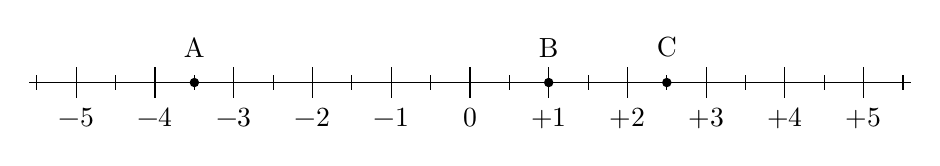
\begin{tikzpicture}
  \draw (-5.6,0)--(5.6,0);
  \foreach \x in {-5,...,0,+1,+2,+3,+4,+5} \draw (\x, 0)--(\x,-0.2)node[below] {$\x$};
  \foreach \x in {-5,...,5} \draw (\x, 0)--(\x,0.2)node[above] {};
  \foreach \x in {-5.5,...,5.5} \draw (\x, 0)--(\x,0.1)node[above] {};
  \foreach \x in {-5.5,...,5.5} \draw (\x, 0)--(\x,-0.1)node[below] {};
  \fill[black] (-3.5,0) circle(0.06);
  \fill[black] (1,0) circle(0.06);
  \fill[black] (2.5,0) circle(0.06);
  \draw (-3.5, 0.2)node[above] {A};
  \draw (1, 0.2)node[above] {B};
  \draw (2.5, 0.2)node[above] {C};
\end{tikzpicture}

\vspace{5mm}

\noindent\fbox{\large\makebox[1em]{\text{\refstepcounter{kaunta}%
\arabic{kaunta}}}} \hspace{1pt}次の数の絶対値を答えなさい。

(1) $+4$ \hspace{5mm} (2) $-5$ \hspace{5mm} (3) $+3.5$ \hspace{5mm} (4) $-\frac{2}{3}$

\vfill

\noindent\fbox{\large\makebox[1em]{\text{\refstepcounter{kaunta}%
\arabic{kaunta}}}} \hspace{1pt}次の各組の数の大小を、不等号を使って表しなさい。

(1) $+3, \quad -5$ \hspace{5mm} (2) $+6,\quad -9, \quad 0$

\vfill

\noindent\fbox{\large\makebox[1em]{\text{\refstepcounter{kaunta}%
\arabic{kaunta}}}} \hspace{1pt}次の計算をしなさい。

(1) $(-6) +(-3)$ \hfill (2) $(-9)+(+8)$ \hfill (3) $(+2) - (+9)$ \hfill (4) $(-6) - (+7)$ 

\vfill

(5) $-7 +3$ \hfill (6) $3 +(-10)$ \hfill (7) $3 -8$ \hfill (8) $-5 - (-9)$

\vfill

(9) $2.4 - 3.5$ \hfill (10) $\frac{3}{4} - (-\frac{5}{12})$ \hfill (11) $-4 + 9 -3$ \hfill (12) $4-7+(-8)$

\vfill

(13) $(-8) + (+5) + (-3) + (+8) + (-1) + (-5) + (+3) + (+3) + (+7) + (-2) + (-8)$

\vfill

\newpage

\noindent\fbox{\large\makebox[1em]{\text{\refstepcounter{kaunta}%
\arabic{kaunta}}}} \hspace{1pt}次の計算をしなさい。

(\text{\refstepcounter{skaunta}%
\arabic{skaunta}})\hspace{2.5pt}$(-4) \times (-8)$ \hspace{30mm} (\text{\refstepcounter{skaunta}%
\arabic{skaunta}})\hspace{2.5pt}$(-18) \div 3$ \hspace{30mm} (\text{\refstepcounter{skaunta}%
\arabic{skaunta}})\hspace{2.5pt}$7 \times (-6)$ 

\vfill

(\text{\refstepcounter{skaunta}%
\arabic{skaunta}})\hspace{2.5pt}$(-12) \div \biggl(-\dfrac{2}{5} \biggl)$ \hspace{30mm} (\text{\refstepcounter{skaunta}%
\arabic{skaunta}})\hspace{2.5pt}$(-2) \times (-9) \times 3$ \hspace{30mm} (\text{\refstepcounter{skaunta}%
\arabic{skaunta}})\hspace{2.5pt}$(-10)^2$

\vfill

(\text{\refstepcounter{skaunta}%
\arabic{skaunta}})\hspace{2.5pt}$(-6) \times 2 \times (-4) \times (-5)$ \hspace{30mm} (\text{\refstepcounter{skaunta}%
\arabic{skaunta}})\hspace{2.5pt}$3 \times (-4^2)$

\vfill

(\text{\refstepcounter{skaunta}%
\arabic{skaunta}})\hspace{2.5pt}$(-14) \times 3 \div \biggl(-\dfrac{7}{4} \biggl)$ \hspace{30mm} (\text{\refstepcounter{skaunta}%
\arabic{skaunta}})\hspace{2.5pt}$15 \div (-9) \div \dfrac{5}{6}$

\vfill

(\text{\refstepcounter{skaunta}%
\arabic{skaunta}})\hspace{2.5pt}$7 + 45 \div (-3)$ \hspace{50mm} (\text{\refstepcounter{skaunta}%
\arabic{skaunta}})\hspace{2.5pt}$(-3) \times 8 - 6 \times (-4)$ 

\vfill

(\text{\refstepcounter{skaunta}%
\arabic{skaunta}})\hspace{2.5pt}$(-2)^3 + (-5) \times 2$ \hspace{50mm} (\text{\refstepcounter{skaunta}%
\arabic{skaunta}})\hspace{2.5pt}$(-6)^2 \div (-9) - 8$

\vfill

(\text{\refstepcounter{skaunta}%
\arabic{skaunta}})\hspace{2.5pt}$9 - 4 \times (5 -8)$ \hspace{50mm} (\text{\refstepcounter{skaunta}%
\arabic{skaunta}})\hspace{2.5pt}$(-12 -8 \times 6) \div (-5)$

\vfill

\newpage

(\text{\refstepcounter{skaunta}%
\arabic{skaunta}})\hspace{2.5pt}$-8x +5x$ \hspace{30mm} (\text{\refstepcounter{skaunta}%
\arabic{skaunta}})\hspace{2.5pt}$6x -x$ \hspace{30mm} (\text{\refstepcounter{skaunta}%
\arabic{skaunta}})\hspace{2.5pt}$8x \times 2$

\vfill 

(\text{\refstepcounter{skaunta}%
\arabic{skaunta}})\hspace{2.5pt}$18y \div (-6)$ \hspace{30mm} (\text{\refstepcounter{skaunta}%
\arabic{skaunta}})\hspace{2.5pt}$(2a -3) - (4a - 7)$ \hspace{30mm} (\text{\refstepcounter{skaunta}%
\arabic{skaunta}})\hspace{2.5pt}$-2(3a + 8)$

\vfill 

(\text{\refstepcounter{skaunta}%
\arabic{skaunta}})\hspace{2.5pt}$(28a - 20) \div 4$ \hspace{50mm} (\text{\refstepcounter{skaunta}%
\arabic{skaunta}})\hspace{2.5pt}$2(2x +3) + 5(x + 1)$ 

\vfill

(\text{\refstepcounter{skaunta}%
\arabic{skaunta}})\hspace{2.5pt}$\dfrac{a + 3}{2} + \dfrac{2a +7}{6}$ \hspace{50mm} (\text{\refstepcounter{skaunta}%
\arabic{skaunta}})\hspace{2.5pt}$18 \times \dfrac{3x -4}{9}$

\vfill

\noindent\fbox{\large\makebox[1em]{\text{\refstepcounter{kaunta}%
\arabic{kaunta}}}} \hspace{1pt}次の方程式を解きなさい。

\setcounter{skaunta}{0}

(\text{\refstepcounter{skaunta}%
\arabic{skaunta}})\hspace{2.5pt}$x - 7 = 6$ \hfill (\text{\refstepcounter{skaunta}%
\arabic{skaunta}})\hspace{2.5pt}$\dfrac{1}{2}x + 3 = x - 1$ \hfill (\text{\refstepcounter{skaunta}%
\arabic{skaunta}})\hspace{2.5pt}$3(x - 2) = 5x - 10$ \hfill (\text{\refstepcounter{skaunta}%
\arabic{skaunta}})\hspace{2.5pt}$x : 3 = 4 : 5$

\vfill

(\text{\refstepcounter{skaunta}%
\arabic{skaunta}})\hspace{2.5pt}$2x + 9 = 5$\hfill (\text{\refstepcounter{skaunta}%
\arabic{skaunta}})\hspace{2.5pt}$2x + 5 = -3x + 10$ \hfill (\text{\refstepcounter{skaunta}%
\arabic{skaunta}})\hspace{2.5pt}$5x + 3 = 2(x - 9)$ 

\vfill

(\text{\refstepcounter{skaunta}%
\arabic{skaunta}})\hspace{2.5pt}$\dfrac{2x - 1}{5} = \dfrac{x - 2}{4}$ \hfill (\text{\refstepcounter{skaunta}%
\arabic{skaunta}})\hspace{2.5pt}$0.005x + 1.2 = 0.16x - 1$ \hfill (\text{\refstepcounter{skaunta}%
\arabic{skaunta}})\hspace{2.5pt}$5 : 6 = 15 : x$ 

\vfill

\newpage

(\text{\refstepcounter{skaunta}%
\arabic{skaunta}})\hspace{2.5pt}$x : (14 -x) = 3 : 4$ \hfill (\text{\refstepcounter{skaunta}%
\arabic{skaunta}})\hspace{2.5pt}$-x + 8 = 3x$ \hfill (\text{\refstepcounter{skaunta}%
\arabic{skaunta}})\hspace{2.5pt}$12y + 1 = 9y + 5$

\vfill

(\text{\refstepcounter{skaunta}%
\arabic{skaunta}})\hspace{2.5pt}$3x - 4(2x - 1) = 29$ \hfill (\text{\refstepcounter{skaunta}%
\arabic{skaunta}})\hspace{2.5pt}$2(x - 1) = 7(- x - 8)$ \hfill (\text{\refstepcounter{skaunta}%
\arabic{skaunta}})\hspace{2.5pt}$1.3 - 0.8x = 0.9 - x$ 

\vfill

(\text{\refstepcounter{skaunta}%
\arabic{skaunta}})\hspace{2.5pt}$\dfrac{3}{2}a - 7 = \dfrac{1}{3}a$ \hfill (\text{\refstepcounter{skaunta}%
\arabic{skaunta}})\hspace{2.5pt}$0.3(0.2x - 1) = 0.54$ \hfill (\text{\refstepcounter{skaunta}%
\arabic{skaunta}})\hspace{2.5pt}$\dfrac{2}{3}x -3 = \dfrac{1}{12}(3x + 4)$

\vfill

(\text{\refstepcounter{skaunta}%
\arabic{skaunta}})\hspace{2.5pt}$(x + 1):3 = 5x :12$ \hfill (\text{\refstepcounter{skaunta}%
\arabic{skaunta}})\hspace{2.5pt}$3x = 21$ \hfill (\text{\refstepcounter{skaunta}%
\arabic{skaunta}})\hspace{2.5pt}$17x = -17$ 

\vfill

(\text{\refstepcounter{skaunta}%
\arabic{skaunta}})\hspace{2.5pt}$18 = -2x$ \hfill (\text{\refstepcounter{skaunta}%
\arabic{skaunta}})\hspace{2.5pt}$\dfrac{x}{7} = 3$ \hfill (\text{\refstepcounter{skaunta}%
\arabic{skaunta}})\hspace{2.5pt}$\dfrac{4x -5}{3} = 2x - 9$

\vfill

\newpage

\setcounter{skaunta}{0}
\noindent\fbox{\large\makebox[1em]{\text{\refstepcounter{kaunta}%
\arabic{kaunta}}}} \hspace{1pt}$y$は$x$に比例し、$x = 3$のとき、$y = -9$です。このとき、次の問に答えなさい。

(\text{\refstepcounter{skaunta}%
\arabic{skaunta}})\hspace{2.5pt}$y$を$x$の式で表しなさい。

\vspace{10mm}

(\text{\refstepcounter{skaunta}%
\arabic{skaunta}})\hspace{2.5pt}次の表を完成させなさい。
\begin{center}
\begin{tabular}{c|ccccccc}
\hline
$x$ & $\cdots$ & $-4$ & $0$ & $4$ & $\cdots$ & $12$ & $\cdots$ \\
\hline
$y$ & $\cdots$ &  &  &  & $\cdots$ & & $\cdots$ \\
\hline
\end{tabular}
\end{center}


(\text{\refstepcounter{skaunta}%
\arabic{skaunta}})\hspace{2.5pt}$x = 2$のときの$y$の値を求めなさい。

\vspace{10mm}

(\text{\refstepcounter{skaunta}%
\arabic{skaunta}})\hspace{2.5pt}$x$の値が増加すると、$y$の値は増加しますか、それとも減少しますか。

\setcounter{skaunta}{0}

\vfill

\noindent\fbox{\large\makebox[1em]{\text{\refstepcounter{kaunta}%
\arabic{kaunta}}}} \hspace{1pt}$y$は$x$に反比例し、$x = 4$のとき、$y = 6$です。このとき、次の問に答えなさい。

(\text{\refstepcounter{skaunta}%
\arabic{skaunta}})\hspace{2.5pt}$y$を$x$の式で表しなさい。

\vspace{10mm}

(\text{\refstepcounter{skaunta}%
\arabic{skaunta}})\hspace{2.5pt}次の表を完成させなさい。

\begin{center}
\begin{tabular}{c|ccccccc}
\hline
$x$ & $\cdots$ & $-4$ & $0$ & $4$ & $\cdots$ & $12$ & $\cdots$ \\
\hline
$y$ & $\cdots$ &  & $\times$ &  & $\cdots$ & & $\cdots$ \\
\hline
\end{tabular}
\end{center}

(\text{\refstepcounter{skaunta}%
\arabic{skaunta}})\hspace{2.5pt}$x = -3$のときの$y$の値を求めなさい。

\vspace{10mm}

(\text{\refstepcounter{skaunta}%
\arabic{skaunta}})\hspace{2.5pt}$x$の変域が正のとき、$x$の値が増加すると、$y$の値は増加しますか、それとも減少しますか。

\vfill

\newpage

\setcounter{skaunta}{0}
\noindent\fbox{\large\makebox[1em]{\text{\refstepcounter{kaunta}%
\arabic{kaunta}}}} \hspace{1pt}次のおうぎ形に関する問に答えなさい。

(\text{\refstepcounter{skaunta}%
\arabic{skaunta}})\hspace{2.5pt}半径が$6\si{cm},$中心角が$\ang{30}$のおうぎ形の面積

\vspace{20mm}

(\text{\refstepcounter{skaunta}%
\arabic{skaunta}})\hspace{2.5pt}半径が$10\si{cm},$中心角が$\ang{108}$のおうぎ形の弧の長さ

\vspace{20mm}

(\text{\refstepcounter{skaunta}%
\arabic{skaunta}})\hspace{2.5pt}弧の長さが$10 \pi,$中心角が$\ang{120}$のおうぎ形の面積

\vspace{20mm}

(\text{\refstepcounter{skaunta}%
\arabic{skaunta}})\hspace{2.5pt}半径が$12\si{cm},$面積が$72 \pi \si{cm}^2$のおうぎ形の中心角

\vspace{20mm}

(\text{\refstepcounter{skaunta}%
\arabic{skaunta}})\hspace{2.5pt}弧の長さが$6 \pi \si{cm}, $中心角が$\ang{120}$のおうぎ形の半径

\vspace{20mm}

(\text{\refstepcounter{skaunta}%
\arabic{skaunta}})\hspace{2.5pt}中心角が$\ang{90} \si{cm},$弧の長さが$9 \pi \si{cm}$のおうぎ形の面積

\vspace{20mm}

\begin{multicols}{2}

\noindent\fbox{\large\makebox[1em]{\text{\refstepcounter{kaunta}%
\arabic{kaunta}}}} \hspace{1pt}右の図形について、次の問に答えなさい。

\setcounter{skaunta}{0}

(\text{\refstepcounter{skaunta}%
\arabic{skaunta}})\hspace{2.5pt}三角形を直線$l$を対称の軸として対称移動させた図形をかきなさい。

\vspace*{\fill}

\columnbreak

\begin{center}
\def\@captype{figure}
\includegraphics[width=30mm]{media/tu4.png}


\end{center}

\end{multicols}

\begin{multicols}{2}

(\text{\refstepcounter{skaunta}%
\arabic{skaunta}})\hspace{2.5pt}三角形を点Oを中心として$\ang{180}$回転移動させた図形をかきなさい。

\vspace*{\fill}

\columnbreak

\begin{center}
\def\@captype{figure}
\includegraphics[width=30mm]{media/image3.png}

\end{center}

\end{multicols}

\newpage

\setcounter{skaunta}{0}

\noindent\fbox{\large\makebox[1em]{\text{\refstepcounter{kaunta}%
\arabic{kaunta}}}} \hspace{1pt}次の作図をしなさい。ただし、作図に用いた線は残しておくこと。

(\text{\refstepcounter{skaunta}%
\arabic{skaunta}})\hspace{2.5pt}$\triangle$ABCで、辺BCを底辺としたときの高さAP

\begin{center}
\def\@captype{figure}
\includegraphics[width=50mm]{media/image10.png}

\end{center}

(\text{\refstepcounter{skaunta}%
\arabic{skaunta}})\hspace{2.5pt}線分ABの中点M

\vspace{30mm}

\begin{center}
\def\@captype{figure}
\includegraphics[width=50mm]{media/image11.png}

\end{center}

(\text{\refstepcounter{skaunta}%
\arabic{skaunta}})\hspace{2.5pt}$\angle$AOBの二等分線OC

\begin{center}
\def\@captype{figure}
\includegraphics[width=50mm]{media/image8.png}

\end{center}

(\text{\refstepcounter{skaunta}%
\arabic{skaunta}})\hspace{2.5pt}線分ABの垂直二等分線

\vspace{30mm}

\begin{center}
\def\@captype{figure}
\includegraphics[width=50mm]{media/image11.png}

\end{center}

(\text{\refstepcounter{skaunta}%
\arabic{skaunta}})\hspace{2.5pt}辺AC, AB, BDに接する円O

\vspace{15mm}

\begin{center}
\def\@captype{figure}
\includegraphics[width=50mm]{media/image191.png}

\end{center}

\newpage

\setcounter{skaunta}{0}
\noindent\fbox{\large\makebox[1em]{\text{\refstepcounter{kaunta}%
\arabic{kaunta}}}} \hspace{1pt}次の立体の体積を求めなさい。

\begin{multicols}{3}

(\text{\refstepcounter{skaunta}%
\arabic{skaunta}})\hspace{2.5pt}

\begin{center}
\def\@captype{figure}
\includegraphics[height=30mm]{img/img7.jpg}

\end{center}

\columnbreak

(\text{\refstepcounter{skaunta}%
\arabic{skaunta}})\hspace{2.5pt}

\begin{center}
\def\@captype{figure}
\includegraphics[height=30mm]{img/img8.jpg}

\end{center}

\columnbreak

(\text{\refstepcounter{skaunta}%
\arabic{skaunta}})\hspace{2.5pt}

\begin{center}
\def\@captype{figure}
\includegraphics[height=30mm]{img/img9.jpg}

\end{center}

\end{multicols}

\vfill

\begin{multicols}{3}

(\text{\refstepcounter{skaunta}%
\arabic{skaunta}})\hspace{2.5pt}

\begin{center}
\def\@captype{figure}
\includegraphics[height=30mm]{img/img10.jpg}

\end{center}

\columnbreak

(\text{\refstepcounter{skaunta}%
\arabic{skaunta}})\hspace{2.5pt}

\begin{center}
\def\@captype{figure}
\includegraphics[height=30mm]{img/img14.jpg}

\end{center}

\columnbreak

(\text{\refstepcounter{skaunta}%
\arabic{skaunta}})\hspace{2.5pt}

\begin{center}
\def\@captype{figure}
\includegraphics[height=30mm]{img/img12.jpg}

\end{center}

\end{multicols}

\vfill

\setcounter{skaunta}{0}
\noindent\fbox{\large\makebox[1em]{\text{\refstepcounter{kaunta}%
\arabic{kaunta}}}} \hspace{1pt}次の立体の表面積を求めなさい。

\begin{multicols}{3}

(\text{\refstepcounter{skaunta}%
\arabic{skaunta}})\hspace{2.5pt}

\begin{center}
\def\@captype{figure}
\includegraphics[height=30mm]{img/img13.jpg}

\end{center}

\columnbreak

(\text{\refstepcounter{skaunta}%
\arabic{skaunta}})\hspace{2.5pt}

\begin{center}
\def\@captype{figure}
\includegraphics[height=30mm]{img/img11.jpg}

\end{center}

\columnbreak

(\text{\refstepcounter{skaunta}%
\arabic{skaunta}})\hspace{2.5pt}

\begin{center}
\def\@captype{figure}
\includegraphics[height=30mm]{img/img12.jpg}

\end{center}

\end{multicols}

\vfill

\newpage

\setcounter{skaunta}{0}

\noindent\fbox{\large\makebox[1em]{\text{\refstepcounter{kaunta}%
\arabic{kaunta}}}} \hspace{1pt}次の資料はあるクラスの生徒10人の数学のテストの点数を表している。

\begin{center}
\begin{tabular}{|cccccccccc|}
\hline
76 & 63 & 84 & 59 & 70 & 84 & 91 & 64 & 82 & 84 \\
\hline
\end{tabular}
\end{center}

\begin{multicols}{2}

(\text{\refstepcounter{skaunta}%
\arabic{skaunta}})\hspace{2.5pt}平均値を求めなさい。

\columnbreak

(\text{\refstepcounter{skaunta}%
\arabic{skaunta}})\hspace{2.5pt}中央値を求めなさい。

\end{multicols}

\vspace{3mm}

\begin{multicols}{2}

(\text{\refstepcounter{skaunta}%
\arabic{skaunta}})\hspace{2.5pt}最瀕値を求めなさい。

\columnbreak

(\text{\refstepcounter{skaunta}%
\arabic{skaunta}})\hspace{2.5pt}範囲を求めなさい。

\end{multicols}

\vspace{3mm}

\begin{multicols}{2}

\setcounter{skaunta}{0}
\noindent\fbox{\large\makebox[1em]{\text{\refstepcounter{kaunta}%
\arabic{kaunta}}}} \hspace{1pt}さやかさんたちは,A中学校とB中学校のどちらのほうが通学時間が長い傾向にあるかを話し合っている。右の表は,A中学校の生徒35人とB中学校の生徒50人の片道の通学時間を,度数分布表に整理したものである。

\columnbreak

\begin{tabular}{|c|c|c|}
\hline
階級(分) & A中学校(人) & B中学校(人)\\
\hline
\footnotesize{以上}\phantom{$\sim$} \footnotesize{未満} & & \\
$0 \sim 10$  & 3 & 6 \\
$10 \sim 20$ & 5 & 9 \\
$20 \sim 30$ & 6 & 11 \\
$30 \sim 40$ & 11 & 12 \\
$40 \sim 50$ & 6 & 7 \\
$50 \sim 60$ & 4 & 5 \\
\hline
合計 & 35 & 50 \\
\hline

\end{tabular}

\end{multicols}

(\text{\refstepcounter{skaunta}%
\arabic{skaunta}})\hspace{2.5pt}階級の幅と最瀕値を答えなさい。

\vfill

(\text{\refstepcounter{skaunta}%
\arabic{skaunta}})\hspace{2.5pt}下の表の空欄を埋めなさい。
\setcounter{kcounter}{0}

\begin{center}

\begin{tabular}{|c|c|c|c|c|}
\hline
階級(分) & A中学校(人) & 相対度数A & B中学校(人)& 相対度数B \\
\hline
\footnotesize{以上}\phantom{$\sim$} \footnotesize{未満} & & & & \\
$0 \sim 10$  & 3 & 0.09 & 6 & \framebox[1.5cm][c]{\raise 0.2ex\hbox{\textcircled{\scriptsize{\refstepcounter{kcounter}\ifthenelse{\value{kcounter}=1}{ア}{\ifthenelse{\value{kcounter}=2}{イ}{\ifthenelse{\value{kcounter}=3}{ウ}{\ifthenelse{\value{kcounter}=4}{エ}{\ifthenelse{\value{kcounter}=5}{オ} {\ifthenelse{\value{kcounter}=6}{カ}{\ifthenelse{\value{kcounter}=7}{キ}{\ifthenelse{\value{kcounter}=8}{ク}{\ifthenelse{\value{kcounter}=9}{ケ}{\ifthenelse{\value{kcounter}=10}{コ}{\ifthenelse{\value{kcounter}=11}{サ}{\ifthenelse{\value{kcounter}=12}{シ}{\ifthenelse{\value{kcounter}=13}{ス}{\ifthenelse{\value{kcounter}=14}{セ}{\ifthenelse{\value{kcounter}=15}{ソ}{\ifthenelse{\value{kcounter}=16}{タ}{\ifthenelse{\value{kcounter}=17}{チ}{\ifthenelse{\value{kcounter}=18}{ツ}{\ifthenelse{\value{kcounter}=19}{テ}{\ifthenelse{\value{kcounter}=20}{ト}{\ifthenelse{\value{kcounter}=21}{ナ}{\ifthenelse{\value{kcounter}=22}{ニ}{\ifthenelse{\value{kcounter}=23}{ヌ}{\ifthenelse{\value{kcounter}=24}{ネ}{\ifthenelse{\value{kcounter}=25}{ノ}{\ifthenelse{\value{kcounter}=26}{ハ}{\ifthenelse{\value{kcounter}=27}{ヒ}{\ifthenelse{\value{kcounter}=28}{フ}{\ifthenelse{\value{kcounter}=29}{ヘ}{\ifthenelse{\value{kcounter}=30}{ホ}{\ifthenelse{\value{kcounter}=31}{マ}{\ifthenelse{\value{kcounter}=32}{ミ}{\ifthenelse{\value{kcounter}=33}{ム}{\ifthenelse{\value{kcounter}=34}{メ}{\ifthenelse{\value{kcounter}=35}{モ}{\ifthenelse{\value{kcounter}=36}{ヤ}{\ifthenelse{\value{kcounter}=37}{ユ}{\ifthenelse{\value{kcounter}=38}{ヨ}{\ifthenelse{\value{kcounter}=39}{ラ}{\ifthenelse{\value{kcounter}=40}{リ}{\ifthenelse{\value{kcounter}=41}{ル}{\ifthenelse{\value{kcounter}=42}{レ}{\ifthenelse{\value{kcounter}=43}{ロ}{\ifthenelse{\value{kcounter}=44}{ワ}{・}}}}}}}}}}}}}}}}}}}}}}}}}}}}}}}}}}}}}}}}}}}}}}}} \\
$10 \sim 20$ & 5 & 0.14 & 9 & 0.18 \\
$20 \sim 30$ & 6 & 0.17 & 11 & 0.22 \\
$30 \sim 40$ & 11 & 0.31 & 12 & \framebox[1.5cm][c]{\raise 0.2ex\hbox{\textcircled{\scriptsize{\refstepcounter{kcounter}\ifthenelse{\value{kcounter}=1}{ア}{\ifthenelse{\value{kcounter}=2}{イ}{\ifthenelse{\value{kcounter}=3}{ウ}{\ifthenelse{\value{kcounter}=4}{エ}{\ifthenelse{\value{kcounter}=5}{オ} {\ifthenelse{\value{kcounter}=6}{カ}{\ifthenelse{\value{kcounter}=7}{キ}{\ifthenelse{\value{kcounter}=8}{ク}{\ifthenelse{\value{kcounter}=9}{ケ}{\ifthenelse{\value{kcounter}=10}{コ}{\ifthenelse{\value{kcounter}=11}{サ}{\ifthenelse{\value{kcounter}=12}{シ}{\ifthenelse{\value{kcounter}=13}{ス}{\ifthenelse{\value{kcounter}=14}{セ}{\ifthenelse{\value{kcounter}=15}{ソ}{\ifthenelse{\value{kcounter}=16}{タ}{\ifthenelse{\value{kcounter}=17}{チ}{\ifthenelse{\value{kcounter}=18}{ツ}{\ifthenelse{\value{kcounter}=19}{テ}{\ifthenelse{\value{kcounter}=20}{ト}{\ifthenelse{\value{kcounter}=21}{ナ}{\ifthenelse{\value{kcounter}=22}{ニ}{\ifthenelse{\value{kcounter}=23}{ヌ}{\ifthenelse{\value{kcounter}=24}{ネ}{\ifthenelse{\value{kcounter}=25}{ノ}{\ifthenelse{\value{kcounter}=26}{ハ}{\ifthenelse{\value{kcounter}=27}{ヒ}{\ifthenelse{\value{kcounter}=28}{フ}{\ifthenelse{\value{kcounter}=29}{ヘ}{\ifthenelse{\value{kcounter}=30}{ホ}{\ifthenelse{\value{kcounter}=31}{マ}{\ifthenelse{\value{kcounter}=32}{ミ}{\ifthenelse{\value{kcounter}=33}{ム}{\ifthenelse{\value{kcounter}=34}{メ}{\ifthenelse{\value{kcounter}=35}{モ}{\ifthenelse{\value{kcounter}=36}{ヤ}{\ifthenelse{\value{kcounter}=37}{ユ}{\ifthenelse{\value{kcounter}=38}{ヨ}{\ifthenelse{\value{kcounter}=39}{ラ}{\ifthenelse{\value{kcounter}=40}{リ}{\ifthenelse{\value{kcounter}=41}{ル}{\ifthenelse{\value{kcounter}=42}{レ}{\ifthenelse{\value{kcounter}=43}{ロ}{\ifthenelse{\value{kcounter}=44}{ワ}{・}}}}}}}}}}}}}}}}}}}}}}}}}}}}}}}}}}}}}}}}}}}}}}}} \\
$40 \sim 50$ & 6 & 0.17 & 7 & 0.14 \\
$50 \sim 60$ & 4 & 0.11 & 5 & \framebox[1.5cm][c]{\raise 0.2ex\hbox{\textcircled{\scriptsize{\refstepcounter{kcounter}\ifthenelse{\value{kcounter}=1}{ア}{\ifthenelse{\value{kcounter}=2}{イ}{\ifthenelse{\value{kcounter}=3}{ウ}{\ifthenelse{\value{kcounter}=4}{エ}{\ifthenelse{\value{kcounter}=5}{オ} {\ifthenelse{\value{kcounter}=6}{カ}{\ifthenelse{\value{kcounter}=7}{キ}{\ifthenelse{\value{kcounter}=8}{ク}{\ifthenelse{\value{kcounter}=9}{ケ}{\ifthenelse{\value{kcounter}=10}{コ}{\ifthenelse{\value{kcounter}=11}{サ}{\ifthenelse{\value{kcounter}=12}{シ}{\ifthenelse{\value{kcounter}=13}{ス}{\ifthenelse{\value{kcounter}=14}{セ}{\ifthenelse{\value{kcounter}=15}{ソ}{\ifthenelse{\value{kcounter}=16}{タ}{\ifthenelse{\value{kcounter}=17}{チ}{\ifthenelse{\value{kcounter}=18}{ツ}{\ifthenelse{\value{kcounter}=19}{テ}{\ifthenelse{\value{kcounter}=20}{ト}{\ifthenelse{\value{kcounter}=21}{ナ}{\ifthenelse{\value{kcounter}=22}{ニ}{\ifthenelse{\value{kcounter}=23}{ヌ}{\ifthenelse{\value{kcounter}=24}{ネ}{\ifthenelse{\value{kcounter}=25}{ノ}{\ifthenelse{\value{kcounter}=26}{ハ}{\ifthenelse{\value{kcounter}=27}{ヒ}{\ifthenelse{\value{kcounter}=28}{フ}{\ifthenelse{\value{kcounter}=29}{ヘ}{\ifthenelse{\value{kcounter}=30}{ホ}{\ifthenelse{\value{kcounter}=31}{マ}{\ifthenelse{\value{kcounter}=32}{ミ}{\ifthenelse{\value{kcounter}=33}{ム}{\ifthenelse{\value{kcounter}=34}{メ}{\ifthenelse{\value{kcounter}=35}{モ}{\ifthenelse{\value{kcounter}=36}{ヤ}{\ifthenelse{\value{kcounter}=37}{ユ}{\ifthenelse{\value{kcounter}=38}{ヨ}{\ifthenelse{\value{kcounter}=39}{ラ}{\ifthenelse{\value{kcounter}=40}{リ}{\ifthenelse{\value{kcounter}=41}{ル}{\ifthenelse{\value{kcounter}=42}{レ}{\ifthenelse{\value{kcounter}=43}{ロ}{\ifthenelse{\value{kcounter}=44}{ワ}{・}}}}}}}}}}}}}}}}}}}}}}}}}}}}}}}}}}}}}}}}}}}}}}}} \\
\hline
合計 & 35 & 1.00 & 50 & 1.00 \\
\hline

\end{tabular}
\end{center}

\vfill

\newpage

(\text{\refstepcounter{skaunta}%
\arabic{skaunta}})\hspace{2.5pt}B中学校の通学時間について、横軸を通学時間、縦軸を相対度数とする、ヒストグラムをかきなさい。

\begin{multicols}{2}

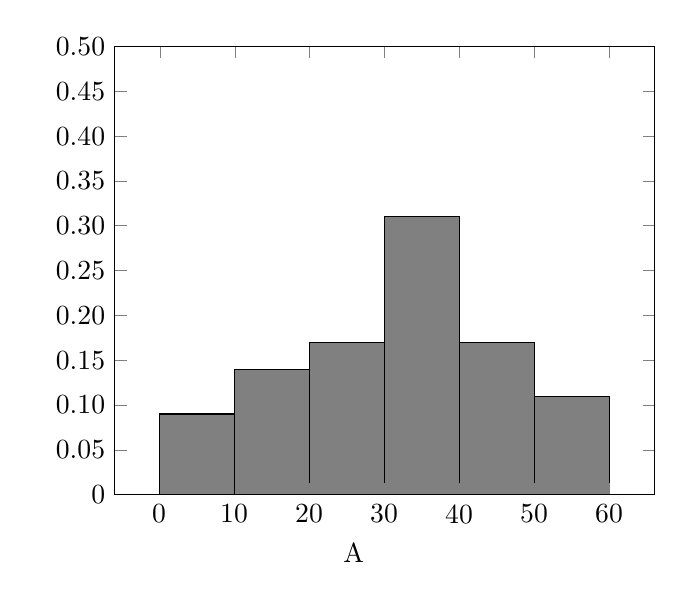
\begin{tikzpicture}
\begin{axis}[ytick={0, 0.05, 0.10, 0.15, 0.20, 0.25, 0.30, 0.35, 0.40, 0.45, 0.50},yticklabels={0, 0.05, 0.10, 0.15, 0.20, 0.25, 0.30, 0.35, 0.40, 0.45, 0.50}, ymax=0.50,ymin=0, area style, xlabel={A中学校の通学時間}, ylabel={相対度数}]
\addplot+[ybar interval, mark=no, fill = {gray}, draw = {black}] plot coordinates { (0, 0.09) (10, 0.14) (20, 0.17) (30, 0.31) (40, 0.17) (50, 0.11) (60, 0.00) };
\end{axis}
\end{tikzpicture}

\columnbreak

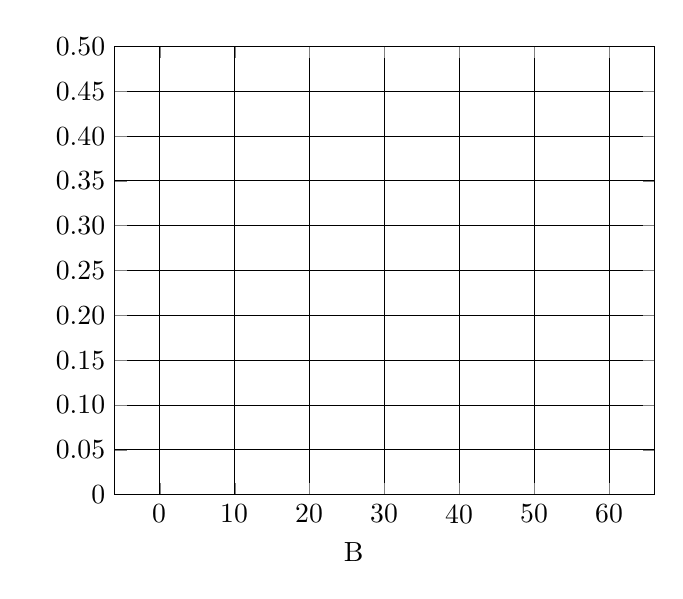
\begin{tikzpicture}
\begin{axis}[ytick={0, 0.05, 0.10, 0.15, 0.20, 0.25, 0.30, 0.35, 0.40, 0.45, 0.50},yticklabels={0, 0.05, 0.10, 0.15, 0.20, 0.25, 0.30, 0.35, 0.40, 0.45, 0.50}, ymax=0.50,ymin=0, area style, xlabel={B中学校の通学時間}, ylabel={相対度数}, grid = both, grid style = {black}]
\addplot+[ybar interval, mark=no] plot coordinates { (0, 0) (10, 0) (20, 0) (30, 0) (40, 0) (50, 0) (60, 0) };
\end{axis}
\end{tikzpicture}

\end{multicols}

\vspace{20mm}

(\text{\refstepcounter{skaunta}%
\arabic{skaunta}})\hspace{2.5pt}B中学校で一人に声をかけて通学時間が40分未満である確率は、どのくらいだと考えられますか。

\vfill

\end{flushleft}

\end{document}
